\documentclass[border=5pt]{standalone}
\usepackage{tikz-qtree}
\begin{document}
\tikzset{every tree node/.style={minimum width=2em,draw,circle},
         blank/.style={draw=none},
         edge from parent/.style=
         {draw, edge from parent path={(\tikzparentnode) -- (\tikzchildnode)}},
         level distance=1cm,
         sibling distance=0.4cm
}
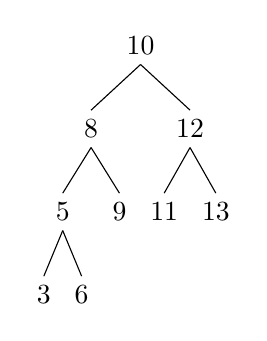
\begin{tikzpicture}
\Tree
[.10
    [.8
        [.5 
            [.3 ]
            [.6 ]
        ]
        [.9 ]
    ]
    [.12  
        [.11 ]
        [.13 ]
]
]
\end{tikzpicture}
\end{document}